% !TEX root = micro_Lie_theory.tex

\section{微型 Lie 理论}

 
%%%%%%%%%%%%%%%%%%%%%%%%%%%%%%%%%%%%%%%%%%%%%%%%%%%%%%%%%%%%%%%%%
\subsection{Lie 群}

\begin{figure}[tb]
\centering
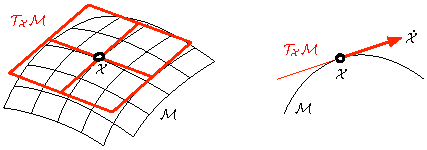
\includegraphics{figures/manifold_tg}
\caption{一个流形 $\cM$ 和向量空间 $\mtanat{\cM}{\cX}$ (在这种情况下 $\cong\bbR^2$)在 $\cX$ 点正切,并有方便的侧切。速度元素, $\dot\cX=\dparil{\cX}{t}$ ,不属于流形 $\cM$ ,但属于切空间 $\mtanat{\cM}{\cX}$。}
\label{fig:manifold_tg}
\end{figure}





在一个唯一的机体中 Lie 群包含群(\emph{group})和光滑流形(\emph{smooth manifold})的概念:Lie群 $\cG$ 是一个光滑流形,其元素满足群公理。
在将这两个概念结合在一起之前,我们将简要介绍这两个概念。

一方面,可微或光滑流形(\emph{smooth manifold})是局部类似于线性空间的拓扑空间。
读者应该能够形象地理解多方面的思想(\figRef{fig:manifold_tg}):它就像一个弯曲的、光滑的(超)表面,没有边缘或尖刺,嵌入到更高维度的空间中。
在机器人学中,我们说我们的状态向量是在这个曲面上演化的,也就是说,流形描述了或是由施加在状态上的约束来定义的。
例如,具有单位范数约束的向量定义半径为$1$的球面流形。
流形的光滑性意味着在每个点上存在唯一的切空间。
这个空间是一个线性或向量空间,我们可以在上面做微积分。 


另一方面,
一个群(\emph{group} $(\cG,\circ)$)是一个集合, $\cG$,具有组合运算, $\circ$,这个算子,对于元素 $\cX,\cY,\cZ\in \cG$,满足下列公理,
%
\begin{align}
\textrm{封闭于 `$\circ$'} & ~:~~ \cX\circ \cY \in \cG  \label{equ:axiom_composition}      \\ 
\textrm{幺元 $\cE$}     & ~:~~ \cE\circ \cX = \cX\circ \cE=\cX  \label{equ:axiom_identity}    \\
\textrm{逆元 $\cX\inv$}    & ~:~~ \cX\inv\circ \cX=\cX\circ \cX\inv=\cE \label{equ:axiom_inverse} \\
\textrm{结合性}      & ~:~~ (\cX\circ \cY)\circ \cZ=\cX\circ(\cY\circ \cZ) 
~.
\end{align}
%


在一个Lie群(\emph{Lie group})中,流形在每一点上看起来都是一样的(例如在球面的表面上,参见 Exs.~\ref{ex:S1} 和 \ref{ex:S3_intro}),并且因此在任意点上的所有切空间都是相同的。
群结构要求流形元素的组合保持在流形上,方程\eqRef{equ:axiom_composition},并且每个元素在流形中也有一个逆元,方程\eqRef{equ:axiom_inverse}。
其中一个特别的元素是幺元,方程\eqRef{equ:axiom_identity},并因此有一个特殊的切空间是幺元处的正切,我们称之为Lie群的Lie代数。
Lie群结合了光滑流形的局部性质,使我们能够利用群的全局性质进行微积分,从而实现远处对象的非线性组合。

% 在本项工作中,为了简单起见,并且在机器人学工作中很常见,我们经常将Lie群称为“流形”。

%
%
\begin{figure}[tb]
\centering
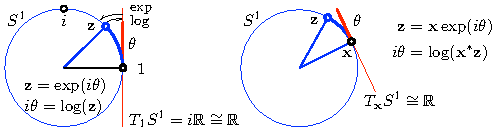
\includegraphics{figures/manifold_z}
\caption{$S^1$ 流形是平面 $\bbC$ 中的单位圆(蓝色),单位复数 $\bfz^*\bfz=1$ 驻留其中。 
Lie代数 $\frak{s}^1=\mtanat{S^1}{\cE}$ 是虚数的线 $i\bbR$ (红色),任意切空间 $\mtan{S^1}$ 都与线 $\bbR$ (红色)同构。
切线向量(红色线段)缠绕流形,形成圆的弧段(蓝色弧段)。
映射 $\exp$ 和 $\log$ 将 $i\bbR$ 的元素(箭头)映射(缠绕和展开)到/自 $S^1$ (蓝色弧段)的元素。
单位复数之间的增量通过组合与指数映射在切线空间中表示(并且我们将为此定义特殊算子 $\op,\om$)。
请参阅正文,以及 \figRef{fig:manifold_q} 所阐述的一个相似的群。
}
\label{fig:manifold_z}
\end{figure}
%

\if\examples y
% !TEX root = micro_Lie_theory.tex


%%%%%%%%%%%%%%%%%%%%%%%%%%%%%  S1  %%%%%%%%%%%%%%%%%%%%%%%%%%%%%%%%
\begin{fexample}	{单位复数群 $S^1$}
\label{ex:S1}

我们的第一个Lie群的例子,是最容易可视化的,是复数乘法下的单位复数群 (\figRef{fig:manifold_z})。
单位复数的形式 $\bfz=\cos\theta+i\sin\theta$。

\emph{-- 作用:}
向量 $\bfx=x+iy$ 在平面内通过复数乘法 $\bfx'=\bfz\,\bfx$ 旋转一个角度 $\theta$。

\emph{-- 群事实:}
单位复数的乘积为单位复数,幺元为 $1$,并且逆元是共轭 $\bfz^*$。

\emph{-- 流形事实:} 
单位范数约束定义了复平面中的单位圆(可以将其视为一维球面,因此命名为 $S^1$)。
这是二维空间中的 1-DoF 曲线。 
单位复数在这个圆上随时间演化。
该群(该圆)在局部重新组装线性空间(切线),而不是在全局重新组装。
\end{fexample}
%%%%%%%%%%%%%%%%%%%%%%%%%%%%%%%%%%%%%%%%%%%%%%%%%%%%%%%%%%%%%%%%%

\fi

\begin{figure}[t]
\centering
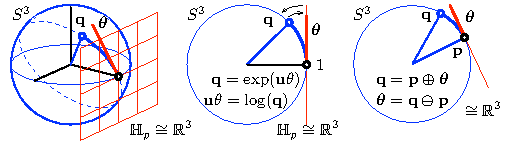
\includegraphics{figures/manifold_q}
\caption{$S^3$ 流形是四元数 $\bbH$ 的四维空间中的单位三维球面(蓝色),单位四元数 $\bfq^*\,\bfq=1$ 驻留其中。
Lie代数是纯虚四元数 $ix+jy+kz\in\bbH_p$ 的空间,同构于超平面 $\bbR^3$ (红色网格),任意其它切空间 $\mtan{S^3}$ 也同构于 $\bbR^3$。
切向量(红色线段)将流形缠绕在大圆弧或测地线(\emph{geodesic})(虚线)上。
中间和右边的图显示了通过该测地线的一个侧切(请注意它与 \figRef{fig:manifold_z} 中的 $S^1$ 有多么相似)。
映射 $\exp$ 和 $\log$ 将 $\bbH_p$ 的元素(箭头)映射(缠绕和展开)到/自 $S^3$ (蓝色弧段)的元素。
四元数之间的增量通过算子 $\op,\om$ 在切空间中表示(参见正文)。
}
\label{fig:manifold_q}
\end{figure}
%
\if\examples y
% !TEX root = micro_Lie_theory.tex

%%%%%%%%%%%%%%%%%%%%%%%%%%%%%  S3  %%%%%%%%%%%%%%%%%%%%%%%%%%%%%%%%
\begin{fexample}	{单位四元数群 $S^3$}
\label{ex:S3_intro}
Lie群的第二个例子,也相对容易可视化,是四元数乘法下的单位四元数群 (\figRef{fig:manifold_q})。
单位四元数的形式 $\bfq=\cos(\theta/2)+\bfu\sin(\theta/2)$,其中 $\bfu=iu_x+ju_y+ku_z$ 是一个单位旋转轴,并且 $\theta$ 是一个旋转角度。

\emph{-- 作用:}
向量 $\bfx=ix+jy+kz$ 在三维空间中通过双四元数乘积 $\bfx'=\bfq\,\bfx\,\bfq^*$ 围绕单位旋转轴 $\bfu$ 旋转一个角度 $\theta$ 。

\emph{-- 群事实:} 
单位四元数的乘积是单位四元数,幺元为 $1$,并且逆元是共轭 $\bfq^*$。

\emph{-- 流形事实:} 
单位范数约束定义了三维球面 $S^3$,一个球形的三维曲面或4维空间中的流形(\emph{manifold})。
在这个曲面上,单位四元数随时间而演变。
该群(该球面)在局部重新组装线性空间(切超平面 $\bbR^3\subset\bbR^4$),而不是在全局重新组装。
\end{fexample}
%%%%%%%%%%%%%%%%%%%%%%%%%%%%%%%%%%%%%%%%%%%%%%%%%%%%%%%%%%%%%

\fi



%%%%%%%%%%%%%%%%%%%%%%%%%%%%%%%%%%%%%%%%%%%%%%%%%%%%%%%%%%%%%%%%%
\subsection{群作用}

重要的是,Lie群具有变换其它集合元素的能力,产生例如旋转、平移、缩放以及它们的组合。 
它们广泛应用于机器人技术中,包括二维和三维。

给定一个Lie群 $\cM$ 和一个集合 $\cV$,我们注意到 $\cX\cdot v$ 是 $v\in\cV$ 上的 $\cX\in\cM$ 的作用($\emph{action}$),
%
\begin{align}
\cdot~:~\cM\times\cV\to\cV~;~ (\cX,v)\mapsto\cX\cdot v
~.
\end{align}
%
对于 $\cdot$ 要成为一个群作用,它必须满足公理, 
%
\begin{align}\label{equ:action}
\textrm{幺元} &:& \cE\cdot v &= v \\
\textrm{相容性} &:& (\cX\circ\cY)\cdot v &= \cX\cdot(\cY\cdot v)
~.
\end{align}


常见的例子有旋转矩阵群 $\SO(n)$,单位四元数群和刚体运动群 $\SE(n)$。
它们各自对向量的作用满足
%
\begin{align*}
\SO(n) &:\textrm{旋转矩阵 } & \bfR\cdot\bfx &\te \bfR\bfx \\
\SE(n) &:\textrm{欧氏矩阵 } & \bfH\cdot\bfx &\te \bfR\bfx + \bft \\
S^1  &:\textrm{单位复数 } & \bfz\cdot\bfx &\te \bfz\,\bfx \\
S^3  &:\textrm{单位四元数 } & \bfq\cdot\bfx &\te \bfq\,\bfx\,\bfq^*
\end{align*}
%
对于更详细的阐述,参见 \tabRef{tab:manifolds} ,以及附录的内容。

% !TEX root = micro_Lie_theory.tex

\begin{table*}[tb]
\caption{二维和三维运动中使用的经典Lie群,包括平凡的 $\bbR^n$。完整参考见附录 
%and the IMU delta composite
}
\label{tab:manifolds}
\begin{center}
\begin{tabular}{|c|c|c|c|c|c|c|c|c|c|c|}
\multicolumn{2}{|c|}{Lie群 $\cM,\circ$} & \!大小\! & \!维度\! 
  & $\cX\in\cM$ 
  & 约束
  & $\bftau^\wedge\in\frak{m}$    
  & $\bftau\in\bbR^m$ 
  & $\Exp(\bftau)$  
  & 组合
  & 作用
  \\
\toprule
%& R^n  ----------------------      
$n$维向量  & $\bbR^n,+$ & $n$  & $n$ 
  & $\bfv\in\bbR^n$ 
  & $\bfv-\bfv=\bf0$
  & $\bfv\in\bbR^n$     
  & $\bfv\in\bbR^n$  
  & $\bfv=\exp(\bfv)$ 
  & $\bfv_1\!+\!\bfv_2$
  & $\bfv + \bfx$
  \\
\midrule
%& S1   ----------------------
圆        & $S^1,\cdot$   & 2    & 1 
  & $\bfz\in\bbC$ 
  & $\bfz^*\bfz=1$
  & $i\theta\in i\bbR$  
  & $\theta\in\bbR$  
  & $\bfz=\exp(i\theta)$ 
  & $\bfz_1\,\bfz_2$
  & $\bfz\,\bfx$
  \\
%& SO(2) ---------------------
旋转   & $\SO(2),\cdot$ & 4    & 1 
  & $\bfR$ 
  & $\bfR\tr\bfR=\bfI$
  & $\hatx{\theta}\in\so(2)$     
  & $\theta\in\bbR$    
  & $\bfR=\exp(\hatx{\theta})$ 
  & $\bfR_1\,\bfR_2$
  & $\bfR\,\bfx$
  \\
%& SE(2)  -------------------- 
刚体运动  
  & $\SE(2),\cdot$ & 9    & 3   
  & $\bfM=\begin{bsmallmatrix}\bfR & \bft \\ 0 & 1\end{bsmallmatrix}$ 
  & $\bfR\tr\bfR=\bfI$
  & $\begin{bsmallmatrix}\hatx{\theta} & \bfrho \\ 0 & 0 \end{bsmallmatrix} \!\in\!\se(2)$     
  & $\begin{bsmallmatrix}\bfrho\\ \theta\end{bsmallmatrix}\in\bbR^3$  
  & $\exp\left(\begin{bsmallmatrix}\hatx{\theta} & \bfrho \\ 0 & 0\end{bsmallmatrix}\right)$ 
  & $\bfM_1\,\bfM_2$
  & $\bfR\,\bfx\!+\!\bft$
  \\
\midrule
%& S3  -----------------------  
三维球面      & $S^3,\cdot$ & 4    & 3   
  & $\bfq\in\bbH$ 
  & $\bfq^*\bfq=1$
  & $\bth/2\in\bbH_p$  
  & $\bth\in\bbR^3$  
  & $\bfq=\exp(\bfu\theta/2)$ 
  & $\bfq_1\,\bfq_2$
  & $\bfq\,\bfx\,\bfq^*$ 
  \\
%& SO(3) ---------------------
旋转   & $\SO(3),\cdot$ & 9    & 3   
  & $\bfR$ 
  & $\bfR\tr\bfR=\bfI$
  & $\hatx{\bth}\in\so(3)$     
  & $\bth\in\bbR^3$  
  & $\bfR=\exp(\hatx{\bth})$ 
  & $\bfR_1\,\bfR_2$
  & $\bfR\,\bfx$
  \\
%& SE(3)  -------------------- 
刚体运动  & $\SE(3),\cdot$   & 16   & 6 
  & $\bfM=\begin{bsmallmatrix}\bfR & \bft \\ 0 & 1\end{bsmallmatrix}$ 
  & $\bfR\tr\bfR=\bfI$
  & $\begin{bsmallmatrix}\hatx{\bth} & \bfrho \\ 0 & 0\end{bsmallmatrix} \!\in\!\se(3)$     
  & $\begin{bsmallmatrix}\bfrho\\\bth\end{bsmallmatrix}\in\bbR^6$  
  & $\exp\left(\begin{bsmallmatrix}\hatx{\bth} & \bfrho \\ 0 & 0\end{bsmallmatrix}\right)$ 
  & $\bfM_1\,\bfM_2$
  & $\bfR\,\bfx\!+\!\bft$
  \\
%\midrule
%% IMU deltas -----------------
%IMU delta     & $\cD,\boxplus$ & 11    & 10 
%  & $\D=\begin{bsmallmatrix}\Dp\\	\Dq \\ \Dv \\ \Dt \end{bsmallmatrix}$ 
%  & $\!\Dq^*\!\Dq\!=\!1\!$
%  & $\begin{bsmallmatrix}\Dp\\	\bfu\Delta\theta/2 \\ \Dv \\ \Dt \end{bsmallmatrix}$ 
%  & $\begin{bsmallmatrix}\Dp\\	\Dth \\ \Dv \\ \Dt \end{bsmallmatrix}\!\in\!\bbR^{10}$  
%  & $\begin{bsmallmatrix}\Dp\\	\exp(\bfu\Dth/2) \\ \Dv \\ \Dt \end{bsmallmatrix}$ 
%  & $\D_1\!\boxplus\!\D_2$
%  & \textrm{---}
%  \\
\bottomrule
\end{tabular}
\end{center}
\end{table*}%



群的组合方程 \eqRef{equ:axiom_composition} 可能被视为群对自身的操作,$\circ:\cM\times\cM\to\cM$。
另一个有趣的作用是伴随作用(\emph{adjoint action}),我们将在 \secRef{sec:adjoint} 看到它。





%%%%%%%%%%%%%%%%%%%%%%%%%%%%%%%%%%%%%%%%%%%%%%%%%%%%%%%%%%%%%%%%%
\subsection{切空间与Lie代数}

给定 $\cX(t)$ 为在Lie群流形 $\cM$ 上移动的点,它的速度 $\dot\cX=\dparil{\cX}{t}$ 属于 $\cX$ 处与 $\cM$ 正切的空间 (\figRef{fig:manifold_tg}),
我们标记为 $\mtanat{\cM}{\cX}$。
流形的光滑性,即没有边或尖峰,意味着在每个点上存在唯一的切空间。
这种切空间的结构在任意地方都是相同的。





%===============================================================
\subsubsection[The Lie algebra]{Lie代数 $\frak{m}$}

幺元 $\mtanat{\cM}{\cE}$ 处的切空间称为 $\cM$ 的Lie代数(\emph{Lie algebra}),标记为 $\frak{m}$,
%
\begin{align}
\textrm{Lie algebra}&:&\frak{m} &\te \mtanat{\cM}{\cE}~.
\end{align}
%
每一个Lie群都有一个关联的Lie代数。
我们通过以下事实 ~\cite{EADE-Lie} 将Lie群与其Lie代数联系起来(参见 Figs.~\ref{fig:exponential} 和 \ref{fig:maps}):
\begin{itemize}
\item
Lie代数 $\frak{m}$ 是一个向量空间。\footnotemark\ 
因此,它的元素可以用 $\bbR^m$ 中的向量来标识(\emph{identified}),其维数 $m$ 是 $\cM$ 的自由度。
\footnotetext{%
在任意Lie代数中,向量空间被赋予一个称为Lie括号的非结合积。在本项工作中,我们不会利用它。}
\item
指数映射(\emph{exponential map}), $\exp:\frak{m}\to\cM$,将Lie代数的元素精确地转化为群的元素。对数映射是逆操作。
\item
通过线性变换, $\cX$ 处的切空间的向量可以变换到幺元 $\cE$ 处的切空间。这种变换称为伴随(\emph{adjoint})变换。
\end{itemize}
%
%


\begin{figure}[tb]
\centering
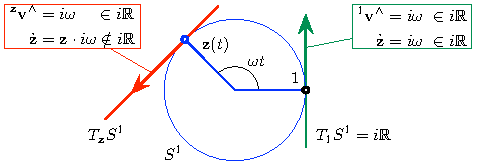
\includegraphics{figures/lie_algebra_S1}
\caption{%
令一个点 $\bfz\in S^1$ 以恒定转速 $\omega$ 移动, $\bfz(t)=\cos\omega t+i\sin\omega t$。
它通过 $1$ 和 $\bfz$ 时的速度分别在 $\mtanat{S^1}{1}$ 和 $\mtanat{S^1}{\bfz}$ 的切空间中。
在 $\mtanat{S^1}{\bfz}$ 的情况下,速度是 $\dot\bfz=\bfz \,i\omega = -\omega\sin\omega t + i\omega\cos\omega t$ 当在全局坐标系中表示时, 并且 ${^\bfz}\!\bfv\hhat=i\omega$ 当在局部表示时。
它们之间的关系为 ${^\bfz}\!\bfv\hhat=\bfz\inv\dot\bfz=\bfz^*\dot\bfz$。
在 $\mtanat{S^1}{1}$ 的情况下,这个关系就是幺元 ${^1}\!\bfv\hhat=\dot\bfz=i\omega$。
显然,所有切空间的结构都是 $i\bbR$,这是Lie代数。
这也是 $\dot\bfz$ 在幺元处的结构,这就是为什么Lie代数被定义为幺元的切空间。
}
\label{fig:global_local_tangent}
\end{figure}


Lie代数可以局部定义到一个切点 $\cX$,建立局部坐标系于 $\mtanat{\cM}{\cX}$
(\figRef{fig:global_local_tangent})。
我们将用“帽子”修饰符来表示Lie代数的元素,例如 $\bfv\hhat$ 表示速度或 $\bftau\hhat=(\bfv t)\hhat=\bfv\hhat t$ 表示一般元素。
还可以添加一个左上标来指定精确的切空间,例如 ${^\cX}\!\bfv\hhat\in\mtanat{\cM}{\cX}$ 和 ${^\cE}\!\bfv\hhat\in\mtanat{\cM}{\cE}$。



通过对群约束方程~\eqRef{equ:axiom_inverse}进行时间微分,Lie代数的结构可以在这里%
%
\if \examples y (参见 Examples~\ref{ex:SO3} 和 \ref{ex:S3}) \else \fi 
%
被找到。
对于乘法群,这将产生新的约束 $\cX\inv\dot\cX + \dot{\cX\inv}\cX = 0$,适用于正切于 $\cX$ 的元素(项 $\dot{\cX\inv}$ 是其逆项的导数) 。
因此,Lie代数的元素的形式是,\footnote{对于加法李群,约束 $\cX-\cX=0$ 区别于 $\dot\cX=\dot\cX$,也就是说,没有约束影响切空间。这意味着切空间与群空间相同。更多细节请参见 \appRef{sec:Tn} 。}
%
\begin{align}\label{equ:tangent_structure}
\bfv\hhat = \cX\inv\dot\cX &= -\dot{\cX\inv}\cX
~.
\end{align}
%



%===============================================================
\subsubsection[The Cartesian vector space]{笛卡尔向量空间 $\bbR^m$}

\begin{figure}[tb]
\centering
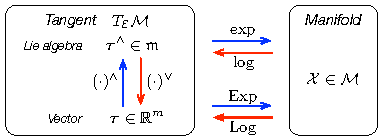
\includegraphics{figures/maps}
\caption{流形 $\cM$ 与其原点 $\mtanat{\cM}{\cE}$ 处的切空间的表示之间的映射(Lie代数 $\frak{m}$ 和笛卡尔 $\bbR^m$)。
映射 hat $(\cdot)\hhat$ 和 vee $(\cdot)\vvee$ 是线性可逆映射或同构(\emph{isomorphisms})方程\eqsRef{equ:hat}{equ:vee},$\exp(\cdot)$ 和 $\log(\cdot)$ 映射 Lie 代数到/自流形,并且 $\Exp(\cdot)$ 和 $\Log(\cdot)$ 是直接将向量空间 $\bbR^m$ 映射到/自 $\cM$ 的快捷方式。}%
\label{fig:maps}%
\end{figure}%


%
Lie代数的元素 $\bftau\hhat$ 具有非平凡结构(斜对称矩阵、虚数、纯虚四元数,参见 \tabRef{tab:manifolds}),
但对我们来说,关键的方面是,它们可以表示为一些基本元素 $E_i$ 的线性组合,其中 $E_i$ 被称为 $\frak{m}$ 的生成元(\emph{generators}) 
(它们是 $\cX$ 在第 $i$ 个方向上围绕原点的导数)。
在 $\bbR^m$ 中将坐标作为向量进行操作是很方便的,我们简单地标记为 $\bftau$。
我们可以从 $\frak{m}$ 传递到 $\bbR^m$ ,反之亦然,通过两个相互逆的线性映射或同构(\emph{isomorphisms}),通常称为 \emph{hat} 和 \emph{vee} (参见 \figRef{fig:maps}),
%
\begin{align} 
\textrm{Hat}&:& 
\bbR^m&\to\frak{m}\,; 
 & 
 \bftau\,
 &\mapsto \bftau\hhat 
 = \sum_{i=1}^m \tau_i\, E_i \label{equ:hat} 
\\
\textrm{Vee}&:& 
 \frak{m}&\to\bbR^m\,; 
 & \bftau\hhat
 & \mapsto (\bftau\hhat)\vvee
 =\bftau
 = \sum_{i=1}^m \tau_i\,\bfe_i  \label{equ:vee}
~,
\end{align}
%
其中 $\bfe_i$ 是 $\bbR^m$ 的基向量(我们有 $\bfe_i\hhat=E_i$)。
这意味着 $\frak{m}$ 与向量空间 $\bbR^m$ 同构 
--- 一个写为 $\frak{m}\cong\bbR^m$, 或者 $\bftau\hhat\cong\bftau$。
对于我们的意图来说,向量 $\bftau\in\bbR^m$ 比它们的同构 $\bftau\hhat\in\frak{m}$ 更易使用,因为它们可以堆叠在更大的状态向量中,更重要的是,可以使用矩阵算子用线性代数进行操作。
在本项工作中,我们实施了 $\bbR^m$ 优于 $\frak{m}$ 的偏好,以至于我们定义的大多数算子和对象(特别是:伴随、Jacobian、扰动及其协方差矩阵,我们很快就会看到)都在 $\bbR^m$ 之上。



\if\examples y
% !TEX root = micro_Lie_theory.tex

%%%%%%%%%%%%%%%%%%%%%%%%%%% SO3 %%%%%%%%%%%%%%%%%%%%%%%%%%%%%%%%%%
\begin{fexample}{旋转群 $\SO(3)$, 它的 Lie 代数 $\so(3)$, 及其向量空间 $\bbR^3$}
\label{ex:SO3}
在 $3\tcross3$ 旋转矩阵 $\bfR$ 的旋转群 $\SO(3)$ 中,我们有正交条件 $\bfR\tr\bfR=\bfI$。
切空间可以通过取该约束的时间导数来找到,即 $\bfR\tr\dot\bfR+\dot\bfR\tr\bfR=0$,我们将其重新排列为 $$\bfR\tr\dot\bfR=-(\bfR\tr\dot\bfR)\tr.$$
这个表达式表明 $\bfR\tr\dot\bfR$ 是一个斜对称矩阵(其转置的负数)。
斜对称矩阵通常用 $\hatx{\bw}$ 表示,其形式如下 
%
$$\hatx{\bw}=\begin{bsmallmatrix}
0 & -\omega_z & \omega_y \\
\omega_z & 0 & -\omega_x \\
-\omega_y & \omega_x & 0 
\end{bsmallmatrix}
.$$
%
这给出 $\bfR\tr\dot\bfR=\hatx{\bw}$。当 $\bfR=\bfI$ 我们有 $$\dot\bfR=\hatx{\bw},$$ 也就是说 $\hatx{\bw}$ 在 $\SO(3)$ 的Lie代数中,我们称之为 $\so(3)$。
%
由于 $\hatx{\bw}\in\so(3)$ 有 $3$ 个自由度, $\SO(3)$ 的维数是 $m=3$。
Lie代数是一个向量空间,它的元素可以分解为
%
$$
\hatx{\bw} = 
  \omega_x\bfE_x+
  \omega_y\bfE_y+
  \omega_z\bfE_z
$$
其中  
$
\bfE_x=
\begin{bsmallmatrix}0&0&0\\0&0&-1\\0&1&0\end{bsmallmatrix}$, 
$\bfE_y=
\begin{bsmallmatrix}0&0&1\\0&0&0\\-1&0&0\end{bsmallmatrix}$,
 $\bfE_z=
\begin{bsmallmatrix}0&-1&0\\1&0&0\\0&0&0\end{bsmallmatrix}$ 
为 $\so(3)$ 的生成元,并且其中 $\bw=(\omega_x,\omega_y,\omega_z)\in\bbR^3$ 是角速度向量。 
%
上面的一对一线性关系允许我们用 $\bbR^3$ 标识 $\so(3)$ --- 我们写为 $\so(3)\cong\bbR^3$。
我们使用线性算子 \emph{hat} 和 \emph{vee} 从 $\so(3)$ 传递到 $\bbR^3$ ,反之亦然,
%
\begin{align*}
\textrm{Hat}&:& \bbR^3&\to\so(3);& \bw&\mapsto\bw^\wedge=\hatx{\bw} 
\\
\textrm{Vee}&:& \so(3)&\to\bbR^3;& \hatx{\bw}&\mapsto\hatx{\bw}^\vee=\bw
~.
\end{align*}
\end{fexample}
%%%%%%%%%%%%%%%%%%%%%%%%%%%%%%%%%%%%%%%%%%%%%%%%%%%%%%%%%%%

\fi



%%%%%%%%%%%%%%%%%%%%%%%%%%%%%%%%%%%%%%%%%%%%%%%%%%%%%%%%%%%%%%%%%
\subsection{指数映射}


\if\examples y
% !TEX root = micro_Lie_theory.tex

%%%%%%%%%%%%%%%%%%%%%%%%% SO3 exp %%%%%%%%%%%%%%%%%%%%%%%%%%%%%%
\begin{fexample}{$\SO(3)$ 的指数映射}
\label{ex:SO3_exp}
%
%We derive here an expression for the exponential map,
%%
%\begin{align*}
%\exp : \so(3)&\to\SO(3);\\
%\hatx{\bth}&\mapsto\exp(\hatx{\bth})
%~.
%\end{align*}
%
我们在 \exRef{ex:SO3} 中看到 
$
\dot\bfR = \bfR\hatx{\bfomega}  \in \mtanat{\SO(3)}{\bfR}.
$
%
对于 $\bw$ 常数,这是一个常微分方程(ODE),其解为 $\bfR(t) = \bfR_0\exp(\hatx{\bfomega}t)$。在原点 $\bfR_0=\bfI$ ,我们有指数映射,
%
\begin{align*}
\bfR(t) &= \exp(\hatx{\bfomega}t) && \in\SO(3)
~. 
\end{align*}
%
我们现在将向量 $\bth\te\bfu\theta \te \bfomega t\in\bbR^3$ 定义为角-轴形式的积分旋转,其中角度 $\theta$ 和单位轴 $\bfu$。 
因此, $\hatx{\bth}\in\so(3)$ 是Lie代数中表示的总旋转。
我们用上面的代换它。 
然后把指数写成幂级数,
%
\begin{align*}
\bfR &= \exp(\hatx{\bth})= \sum_k\frac{\theta^k}{k!}{(\hatx{\bfu})^k} 
~.
\end{align*}
%
为了找到一个封闭形式的表达式,我们写下 $\hatx{\bfu}$ 的几次幂,
%
\begin{align*}
\hatx{\bfu}^0&= \bfI,
&
\hatx{\bfu}^1&= \hatx{\bfu},
\\
\hatx{\bfu}^2&= \bfu\bfu\tr -\bfI,
&
\hatx{\bfu}^3&=-\hatx{\bfu},
\\
\hatx{\bfu}^4&=-\hatx{\bfu}^2,
&
\cdots
\end{align*}
%
并意识到,所有这些都可以表示为 $\bfI$、$\hatx{\bfu}$ 或 $\hatx{\bfu}^2$ 的倍数。
因此,我们将这个级数改写为,
%We substitute them in the series, and group the terms according to the nature of the powers, 
%
\begin{align*}
\bfR = \bfI &+ \hatx{\bfu}\big(\theta - \tfrac1{3!}\theta^3 + \tfrac1{5!}\theta^5 - \cdots\big) \\
  &+ \hatx{\bfu}^2\big(\tfrac12\theta^2-\tfrac1{4!}\theta^4+\tfrac1{6!}\theta^6-\cdots\big)
  ~,
\end{align*}
%
其中,我们确定了 $\sin\theta$ 和 $\cos\theta$ 的级数,得到了封闭形式,
%
\begin{align*}
\bfR=\exp(\hatx{\bfu\theta}) &= 
\bfI + \hatx{\bfu}\sin\theta + \hatx{\bfu}^2(1\!-\!\cos\theta)
~.
\end{align*}
%
这个表达式是众所周知的Rodrigues旋转公式。
它可以用作大写指数方程,只需这么操作 $\bfR=\Exp(\bfu\theta)=\exp(\hatx{\bfu\theta})$。
\end{fexample}
%%%%%%%%%%%%%%%%%%%%%%%%%%%%%%%%%%%%%%%%%%%%%%%%%%%%%

\fi

指数映射 $\exp()$ 允许我们精确地将Lie代数的元素变换到群(\figRef{fig:exponential})上,一般称为收回(\emph{retraction})操作。
直观地说, $\exp()$ 将切元素缠绕在大圆弧或测地线(\emph{geodesic})跟随的流形上(就像将弦缠绕在球上一样, Figs.~\ref{fig:exponential}, \ref{fig:manifold_z} 和 \ref{fig:manifold_q})。
反向映射是 $\log()$,即展开操作。
 $\exp()$ 映射通过考虑流形上 $\cX\in\cM$ 的时间导数自然产生,如下所示。
%
从方程 \eqRef{equ:tangent_structure} 我们有,
%
\begin{align}\label{equ:ode}
\dot\cX &= \cX\bfv\hhat 
~.
\end{align}
%
对于 $\bfv$ 为常数,这是一个常微分方程(ODE),其解是 
%
\begin{align}\label{equ:exp_at_X}
\cX(t)  = \cX(0)\exp(\bfv\hhat t)
~.
\end{align}
%
因为 $\cX(t)$ 和 $\cX(0)$ 是群的元素,所以 $\exp(\bfv\hhat t)=\cX(0)\inv\cX(t)$ 也必须在群中,所以 $\exp(\bfv\hhat t)$ 将Lie代数的元素 $\bfv\hhat t$ 映射到群中。
这被称为指数映射(\emph{exponential map})。

为了给指数映射提供一个更通用的定义,让我们定义切增量 $\bftau\te\bfv t\in\bbR^m$ 作为每一时刻的速度,这样我们就有 $\bftau\hhat=\bfv\hhat t\in\frak{m}$ 做为Lie代数中的一个点。
指数映射和它的逆、对数映射,现在可以写成,
%
\begin{align}
\exp &:& \frak{m} & \to\cM      
 &&; & \bftau\hhat &\mapsto \,\cX = \exp(\bftau\hhat) 
 \\
\log &:&     \cM & \to\frak{m} 
 &&; & \cX\,    &\mapsto \bftau\hhat = \log(\cX) ~
~. 
\end{align}


通过写出绝对收敛的泰勒级数,得到了乘法群中指数的封闭形式,
%
\begin{align}
\exp(\bftau\hhat)=\cE+\bftau\hhat+\tfrac12{\bftau\hhat}^2+\tfrac1{3!}{\bftau\hhat}^3+\cdots
~,
\end{align}
%
并且利用 $\bftau\hhat$ 的幂的代数性质%
\if \examples y (对于指数映射在 $\SO(3)$ 和 $S^3$ 中的扩展参见 Ex.~\ref{ex:SO3_exp} 和 \ref{ex:S3})。 \else. \fi
然后将这些求逆以找到对数映射。
%
指数映射的关键性质是 
%
\begin{align}
\exp((t+s)\bftau\hhat) 
 &= \exp(t\bftau\hhat)\exp(s\bftau\hhat) \label{equ:prop_exp_ts}
 \\
\exp(t\bftau\hhat) 
 &= \exp(\bftau\hhat)^t \label{equ:prop_exp_t}
 \\
\exp(-\bftau\hhat) 
 &= \exp(\bftau\hhat)\inv \label{equ:prop_exp_inv}
 \\
\exp(\cX\bftau\hhat\cX\inv) 
 &= \cX\exp(\bftau\hhat)\cX\inv ~, \label{equ:prop_exp}
\end{align} 
%
其中方程 \eqRef{equ:prop_exp},这是一个惊奇而有力的说明,可以通过扩展泰勒级数和简化许多项 $\cX\inv\cX$ 来轻易地证明。

\if\examples y
% !TEX root = micro_Lie_theory.tex

%%%%%%%%%%%%%%%%%%%% S3 cont %%%%%%%%%%%%%%%%%%%%%%%%%%%%%%%%%
\begin{fexample}{单位四元数群 $S^3$ (条件)}
\label{ex:S3}
在 $S^3$ 群中(回想 \exRef{ex:S3_intro} 并参见 \eg\ \cite{SOLA-17-Quaternion}),单位范数条件 $\bfq^*\bfq=1$ 的时间导数产生 
%
$$\bfq^*\dot\bfq=-(\bfq^*\dot\bfq)^*
.
$$
%
这表明 $\bfq^*\dot\bfq$ 是一个纯虚四元数(其实部为零)。
%The set of pure quaternions is noted $\bbH_p$.
纯虚四元数 $\bfu v\in\bbH_p$ 有形式 
%
$$\bfu v=(iu_x+ju_y+ku_z)v =iv_x+jv_y+kv_z 
,$$
%
其中, $\bfu\te iu_x+ju_y+ku_z$ 是纯幺正的, $v$ 是范数,并且 $i,j,k$ 是Lie代数 $\frak{s}^3=\bbH_p$ 的生成元。
%
重写我们上面的条件,
%
\begin{align*}
\dot\bfq=\bfq\, \bfu v &&\in \mtanat{S^3}{\bfq}
,
\end{align*}
% 
那将积分到 $\bfq = \bfq_0\exp(\bfu v t)$。 
令 $\bfq_0=1$ 并定义 $\bphi \te \bfu\phi \te\bfu v t$ 我们得到指数映射,
%
\begin{align*}
\bfq = \exp(\bfu\phi) \te \sum \frac{\phi^k}{k!}\bfu^k &&\in S^3
~.
\end{align*}
%
$\bfu$ 的幂跟随以下模式 $1,\bfu,-1,-\bfu,1,\cdots$。
因此,我们将项分组为 $1$ 和 $\bfu$ ,并标识 $\cos\phi$ 和 $\sin\phi$ 的级数。
我们得到封闭形式,
%
\begin{align*}
\bfq = \exp(\bfu\phi) = \cos(\phi) + \bfu\sin(\phi) 
~,
\end{align*}
%
这是欧拉公式的优美扩展, $\exp(i\phi)=\cos\phi+i\sin\phi$。
%
Lie代数 $\bfphi=\bfu \phi\in\frak{s}^3$ 的元素可以通过映射 \emph{hat} 和 \emph{vee} 用旋转向量 $\bth\in\bbR^3$ 标识,
%
\begin{align*}
\textrm{Hat}&:& \bbR^3&\to\frak{s}^3;& \bth&\mapsto\bth^\wedge=2\bphi
\\
\textrm{Vee}&:& \frak{s}^3&\to\bbR^3;& \bphi&\mapsto\bphi^\vee=\bth/2
~,
\end{align*}
%
其中 %$\bth \te \bfu\theta\te\bw t$ is the angle-axis vector, and 
因子 $2$ 说明了旋转作用中四元数的双重效应, $\bfx'=\bfq\,\bfx\,\bfq^*$。 
%
通过选择 Hat 和 Vee,四元数指数
%
\begin{align*}
\bfq = \Exp(\bfu\theta)=\cos(\theta/2)+\bfu\sin(\theta/2)
\end{align*}
%
等价于旋转矩阵 $\bfR=\Exp(\bfu\theta)$。
\end{fexample}
%%%%%%%%%%%%%%%%%%%%%%%%%%%%%%%%%%%%%%%%%%%%%%%%%%%%%%%%

\fi



%===============================================================
\subsubsection[The capitalized Exp map]{大写指数映射}


大写的 Exp 和 Log 映射是将向量元素 $\bftau\in\bbR^m~(\cong\mtanat{\cM}{\cE})$ 直接映射到元素 $\cX\in\cM$ 的快捷方式。
% 
我们有,
%
\begin{align}
\Exp &: &\bbR^m &\to\cM &&;&
\,\bftau &\mapsto \cX = \Exp(\bftau)\\
\Log  &: & \cM &\to\bbR^m &&;&
 \cX &\mapsto \bftau\,=\Log(\cX) 
\,. 
\end{align}
%
显然来自 \figRef{fig:maps},
%
\begin{align}
\cX  = \Exp(\bftau) &\te \exp(\bftau\hhat) \\
\bftau =\Log(\cX)    &\te \log(\cX)\vvee 
~. 
\end{align}
%
对于不同流形的这些映射的实现的详细信息,参见附录。


%===============================================================
\subsection{加号和减号算子}

加号和减号算子允许我们在(弯曲的)流形中的元素之间引入增量,并在(平坦的)切向量空间中表示它们。
它们用 $\op$ 和 $\om$表示,将一个 Exp/Log 操作与一个结合操作组合在一起。
由于组合的非交换性,它们根据操作数的顺序在右结合(right-)版本和左结合(left-)版本中定义。
右结合(right-)算子是 (参见 \figRef{fig:manifold_q}-\emph{right}), 
%
\begin{align}
\textrm{right-}\op:&& \cY &= \cX\op{^\cX\!\bftau} \te \cX\circ\Exp({^\cX\!\bftau}) \,\in \cM \label{equ:rplus} \\
\textrm{right-}\om:&& {^\cX\!\bftau} &= \cY\om\cX \,\te \Log(\cX\inv\!\circ\!\cY)\in\mtanat{\cM}{\cX} \label{equ:rminus}
~.
\end{align}
%
因为在方程 \eqRef{equ:rplus} 中 $\Exp({^\cX\!\bftau})$ 出现在组合的右手侧,
${^\cX\!\bftau}$ 属于 $\cX$ 处的切空间(参见方程 \eqRef{equ:rminus}): 
我们按照约定\footnotemark~说这个 ${^\cX\!\bftau}$ 是在 $\cX$ 处的局部(\emph{local})坐标系中表示 --- 我们标记到参考坐标系的左上标。

左结合(left-)算子是
\begin{align}
\textrm{left-}\op:&&\cY&={^\cE\!\bftau}\op\cX \te \Exp({^\cE\!\bftau})\circ\cX \in \cM \label{equ:lplus} \\
\textrm{left-}\om:&&{^\cE\!\bftau}&=~\cY\om\cX \te \Log(\cY\!\circ\!\cX\inv)\in\mtanat{\cM}{\cE}
\label{equ:lminus}
~.
\end{align}
%
现在,在方程 \eqRef{equ:lplus} 中 $\Exp({^\cE\!\bftau})$ 在左侧,并且我们有 ${{^\cE\!\bftau}\in\mtanat{\cM}{\cE}}$:我们说这个 ${{^\cE}\!\bftau}$ 是在全局(\emph{global})坐标系中表示。

请注意,虽然右结合(right-)和左结合(left-)算子 $\op$ 是按操作数顺序区分的,但符号 $\om$ 在方程 \eqRef{equ:rminus} 和 \eqRef{equ:lminus} 中是不明确的。
在本项工作中,我们默认表示局部扰动,因此我们默认使用 $\op$ 和 $\om$ 的右结合(right-)形式。
\footnotetext{这个约定坚持坐标系变换,例如${^G\!\bfx=\bfR^L\!\bfx}$,其中 $\bfR\in \SO(3)$ 将局部向量变换为全局向量。
请注意,并非所有作者都共享此约定,例如文献 \cite{GALLEGO-13} 使用了相反的约定, ${^L\!\bfx=\bfR^G\!\bfx}$。}


%===============================================================
\subsection[Adjoint, and adjoint matrix]{伴随和伴随矩阵}
\label{sec:adjoint}

\begin{figure}[tb]
\centering
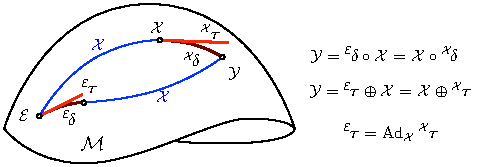
\includegraphics{figures/adjoint}
\caption{两条路径, $\cX\circ{^\cX}\!\delta$ 和 ${^\cE}\!\delta\circ\cX$ ,将原点 $\cE$ 与点 $\cY$ 连接。
它们都用增量或 `deltas' 组成元素 $\cX$ ,在局部坐标系中表示,${^\cX}\!\delta$,或在原点表示, ${^\cE}\!\delta$。
由于非交换性,元素 ${^\cX}\!\delta$ 和 ${^\cE}\!\delta$ 不相等。 
它们的相关切向量 ${^\cX}\!\bftau=\Log({^\cX}\!\delta)$ 和 ${^\cE}\!\bftau=\Log({^\cE}\!\delta)$ 也不相等。
它们联系在一起通过线性变换 ${^\cE}\!\bftau=\Ad[\cM]{\cX}\,{^\cX}\!\bftau$ 其中
$\Ad{\cX}$ 是 $\cM$ 在 $\cX$ 处的伴随。 
}
\label{fig:adjoint}
\end{figure}


如果我们在方程 \eqssRef{equ:rplus,equ:lplus} 中标识 $\cY$ ,我们就得到 ${{^\cE\!\bftau}\op\cX} = {\cX\op{^\cX\!\bftau}}$ ,它确定局部切元素和全局切元素之间的关系 (\figRef{fig:adjoint})。
我们用方程 \eqssRef{equ:prop_exp,equ:rplus,equ:lplus} 来扩展它为
%
\begin{align*}
\Exp({^\cE}\!\bftau)\cX 
 &= \cX\Exp({^\cX}\!\bftau) \\
\exp({^\cE}\!\bftau\hhat) 
 &= \cX \exp({^\cX}\!\bftau\hhat) \cX\inv 
  = \exp(\cX {^\cX}\!\bftau\hhat \cX\inv) \\
{^\cE}\!\bftau\hhat 
 &= \cX {^\cX}\!\bftau\hhat \cX\inv 
\end{align*}
%
\subsubsection{伴随}
因此,我们将 $\cM$ 在 $\cX$ 处的伴随(\emph{adjoint}),记为 $\Adh[\cM]{\cX}$,定义为 
%
\begin{align}
\Adh{\cX}:\frak{m}\to\frak{m};~~ \bftau\hhat\mapsto \Adh[\cM]{\cX}(\bftau\hhat) \te \cX \bftau\hhat \cX\inv \label{equ:Adjh1} 
~,
\end{align}
%
因此 ${^\cE}\!\bftau\hhat = \Adh[\cM]{\cX}({^\cX}\!\bftau\hhat)$。 
这定义了群在它自己的Lie代数上的伴随作用(\emph{adjoint action})。
伴随有两个有趣的(并且很容易证明的)性质,
%
\begin{align*}
\textrm{Linear} &:& \Adh{\cX}(a\bftau\hhat+b\bfsigma\hhat) =& ~a\Adh{\cX}(\bftau\hhat)\\
&&&+b\Adh{\cX}(\bfsigma\hhat) 
\\
\textrm{Homomorphism} &:& \Adh{\cX}(\Adh{\cY}(\bftau\hhat)) =& ~\Adh{\cX\cY}(\bftau\hhat) 
~.
\end{align*}
%
\subsubsection{伴随矩阵}
因为 $\Adh{\cX}()$ 是线性的,我们可以找到一个等价的矩阵算子 $\Ad{\cX}$ ,它映射笛卡尔切向量 ${^\cE}\!\bftau\cong{^\cE}\!\bftau\hhat$ 和 ${^\cX}\!\bftau\cong{^\cX}\!\bftau\hhat$,
%
\begin{align}
\Ad{\cX}:\bbR^m\to\bbR^m;~~ ^\cX\!\bftau\mapsto {^\cE}\!\bftau &= \Ad[\cM]{\cX}{^\cX}\!\bftau \label{equ:Adj2} 
~,
\end{align}
%
我们称之为伴随矩阵(\emph{adjoint matrix})。这可以通过将 $\vvee$ 应用于方程 \eqRef{equ:Adjh1} 来计算,因此写为
%
\begin{align}\label{equ:Adj4} 
\Ad[\cM]{\cX}\,\bftau &= (\cX\bftau\hhat\cX\inv)\vvee 
~,
\end{align}
%
然后扩展右手侧结合以标识伴随矩阵 (参见 Ex.~\ref{ex:SE3_adjoint} 和附录)。
伴随矩阵的其它性质是,
%
\begin{align}
\cX\op\bftau &= (\Ad[\cM]{\cX}\,\bftau)\op\cX \label{equ:Adj1} \\
\Ad[\cM]{\cX\inv} &= \Ad[\cM]{\cX}\inv \label{equ:Adj5} \\
\Ad[\cM]{\cX\cY} &=\Ad[\cM]{\cX}\Ad[\cM]{\cY} \label{equ:Adj7}
~.
\end{align}
%
请注意在方程 \eqssRef{equ:Adj5,equ:Adj7} 中的左半部分通常比右半部分计算起来更便宜。
我们将经常使用伴随矩阵将 $\cX$ 处的切空间的向量线性变换为原点的切空间的向量,使用 ${^\cE}\!\bftau = \Ad{\cX}{^\cX}\!\bftau$ ,方程~\eqRef{equ:Adj2}。
在本项工作中,伴随矩阵将被简单的称为伴随。



\if\examples y
% !TEX root = micro_Lie_theory.tex

%%%%%%%%%%%%%%%%%%%% SE3 adjoint %%%%%%%%%%%%%%%%%%%%%%%%%%%%
\begin{fexample}{$\SE(3)$ 的伴随矩阵}\label{ex:SE3_adjoint}
%
刚体运动的 $\SE(3)$ 群(参见 \appRef{sec:SE3})有群,Lie代数和向量元素,
%
\begin{align*}
\bfM&=\begin{bmatrix}\bfR&\bft\\\bf0&1\end{bmatrix}
~,
&
\bftau\hhat&=\begin{bmatrix}\hatx{\bth}&\bfrho\\\bf0&0\end{bmatrix}
~,
&
\bftau &=\begin{bmatrix}\bfrho\\\bth\end{bmatrix}
~.
\end{align*}
%
伴随矩阵由扩展的方程 \eqRef{equ:Adj4} 标识为
%
\begin{align*}
\Ad{\bfM}\,\bftau
  &= (\bfM\bftau\hhat\bfM\inv)\vvee = \cdots =
  \\
  &= \left(\begin{bmatrix}\bfR\hatx{\bth}\bfR\tr & -\bfR\hatx{\bth}\bfR\tr\bft + \bfR\bfrho \\ \bf0 & \bf0\end{bmatrix}\right)\vvee \\
%  &= \left(\begin{bmatrix}\hatx{\bfR\bth} & -\hatx{\bfR\bth}\bft + \bfR\bfrho \\ \bf0 & \bf0\end{bmatrix}\right)\vvee \\
  &= \left(\begin{bmatrix}\hatx{\bfR\bth} & \hatx{\bft}\bfR\bth + \bfR\bfrho \\ \bf0 & \bf0\end{bmatrix}\right)\vvee \\
  &= \begin{bmatrix}\hatx{\bft}\bfR\bth + \bfR\bfrho \\ \bfR\bth\end{bmatrix} 
%  \\
%  &
  = \begin{bmatrix}\bfR & \hatx{\bft}\bfR\\ \bf0&\bfR\end{bmatrix}\begin{bmatrix}\bfrho \\ \bth\end{bmatrix} 
\end{align*}
%
其中我们使用 $\hatx{\bfR\bth}=\bfR\hatx{\bth}\bfR\tr$ 和 $\hatx{\bfa}\bfb=-\hatx{\bfb}\bfa$ 。所以伴随矩阵是 
%
\begin{align*}
\Ad{\bfM} =  \begin{bmatrix}\bfR & \hatx{\bft}\bfR \\ \bf0&\bfR\end{bmatrix} \quad\in\bbR^{6\times6}
~.
\end{align*}
%
\end{fexample}		
%%%%%%%%%%%%%%%%%%%%%%%%%%%%%%%%%%%%%%%%%%%%%%%%%%%%%%%%%%%%%%%%%

\fi




%%%%%%%%%%%%%%%%%%%%%%%%%%%%%%%%%%%%%%%%%%%%%%%%%%%%%%%%%%%%%%%%%
\subsection{Lie群上的导数}

在Lie群中定义导数的各种方法中,我们主要关注Jacobian矩阵映射向量切空间的形式。 
这在这里就足够了,因为在这些空间中,不确定性和增量可以被恰当而容易地定义。
利用这些Jacobian矩阵,Lie群中的不确定性管理公式与向量空间中的不确定性管理公式基本相似。

下文描述的Jacobian矩阵满足链式规则,因此我们可以很容易地从部分的Jacobian矩阵块的求逆(\emph{inversion})、组合(\emph{composition})、求幂(\emph{exponentiation})和作用(\emph{action})等操作来计算任意Jacobian矩阵。
详情和证明参见 \secRef{sec:jacs_chain_rule} 。


%=======================================================
\subsubsection[Jacobians on vector spaces]{提醒:向量空间上的Jacobian矩阵}

对于多元函数 $f:\bbR^m\to\bbR^n$,Jacobian矩阵定义为所有偏导数的 $n\times m$ 矩阵, 
%
\begin{align}\label{equ:jac_Rn_matrix}
\bfJ = \dpar{f(\bfx)}{\bfx} &\te \begin{bmatrix}
\dpar{f_1}{x_1} & \cdots & \dpar{f_1}{x_m} \\
\vdots && \vdots \\
\dpar{f_n}{x_1} & \cdots & \dpar{f_n}{x_m} 
\end{bmatrix} \in\bbR^{n\times m}
~.
\end{align}
%
用下面的形式定义这个矩阵很方便。让我们分割 $\bfJ=[\bfj_1\cdots\bfj_m]$,并让 $\bfj_i=[\dpar{f_1}{x_i}\cdots\dpar{f_n}{x_i}]\tr$ 作为它的第 $i$ 个列向量。此列向量响应于
%
\begin{align}\label{equ:jac_Rn_i}
\bfj_i = \dpar{f(\bfx)}{x_i} \te \lim_{h\to0}\frac{f(\bfx+h\bfe_i)-f(\bfx)}{h} \in \bbR^n
~,
\end{align}
%
其中 $\bfe_i$ 是 $\bbR^m$ 的自然基的第 $i$ 个向量。
至于分子,注意这个向量 
%
\begin{align}\label{equ:jac_Rn_vec}
\bfv_i(h) \te f(\bfx+h\bfe_i)-f(\bfx) \quad \in\bbR^n
\end{align}
%
是当 $\bfx$ 在 $\bfe_i$ 方向上受到扰动时, $f(\bfx)$ 的变化量,并且相应的Jacobian矩阵的列仅为 $\bfj_i=\dparil{\bfv_i(h)}{h}|_{h=0}=\lim_{h\to0}\bfv_i(h)/h$。
在本项工作中,为了方便起见,我们引入了紧凑形式,
%
\begin{align}\label{equ:jac_Rn}
\mjac{}{}=\dpar{f(\bfx)}{\bfx}\te\lim_{\bfh\to0}\frac{f(\bfx+\bfh)-f(\bfx)}{\bfh}
\in\bbR^{n\times m}
~,
\end{align}
%
其中 $\bfh\in\bbR^m$, 其用方程 \eqRef{equ:jac_Rn_i} 计算所有列
以形成方程 \eqRef{equ:jac_Rn_matrix} 的定义。
我们注意到方程 \eqRef{equ:jac_Rn} 只是一个方便的符号 (就像方程 \eqRef{equ:jac_Rn_matrix} 一样),因为向量 $\bfh$ 的除法未定义,正确的计算需要方程 \eqRef{equ:jac_Rn_i} 。
然而,通过将分子扩展成 $\bfh$ 中的线性形式,并将左手侧标识为Jacobian矩阵,该形式可用于计算Jacobian矩阵,即,
%
\begin{align}\label{equ:jac_Rn_identify}
 \lim_{\bfh\to0}\frac{f(\bfx\!+\!\bfh)\!-\!f(\bfx)}{\bfh} 
 = \cdots
 = \lim_{\bfh\to0}\frac{\bfJ\bfh}{\bfh}  
 \te \dpar{\bfJ\bfh}{\bfh} 
 = \bfJ.
\end{align}
%
最后请注意,对于 $\bfh$ 的小值,我们有线性近似值,
%
\begin{align}
f(\bfx+\bfh) \xrightarrow[\bfh\to0]{} f(\bfx) + \dpar{f(\bfx)}{\bfx}\bfh
~.
\end{align}

%=======================================================
\subsubsection{Lie 群上的右Jacobian矩阵}


\begin{figure}[tb]
\centering
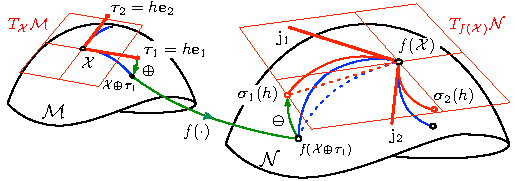
\includegraphics{figures/jacobian}
\caption{函数的右Jacobian矩阵 $f:\cM\to\cN$ 。
正则方向上的扰动向量, $\bftau_i=h\bfe_i\in\mtanat{\cM}{\cX}$,通过加号、应用 $f()$ 和减号(绿色箭头)的过程传播到 $\bfsigma_i\in\mtanat{\cN}{f(\cX)}$ 中的扰动向量,获得 $\bfsigma_i(h)=f(\cX\op h\bfe_i)\om f(\cX)$。 
对于 $h$ 的不同值,请注意,在 $\cM$ 中,扰动 $\bftau_i(h)=h\bfe_i$ (粗红色)沿测地线产生 $\cM$ (蓝色)路径(回忆~\figRef{fig:exponential})。
另请注意,在 $\cN$ 中,由于 $f(\cdot)$ 的非线性,图像路径(蓝色实线)通常不在测地线中(蓝色虚线)。
这些图像路径被提升到切空间 $\mtanat{\cN}{f(\cX)}$,生成平滑的曲线路径(细红色实线)。
$\bfJ$ (粗红线)的列向量 $\bfj_i$ 是在 $f(\cX)$ 处计算的提升路径的导数,
即 $\bfj_i=\lim_{h\to0}\bfsigma_i(h)/h$ 。
每一个 $h\bfe_i\in\mtanat{\cM}{\cX}$ 让位给一个 $\bfj_i\in\mtanat{\cN}{f(\cX)}$,并由此产生的Jacobian矩阵 $\bfJ=[\,\bfj_1\cdots\bfj_m\,]\in\bbR^{n\times m}$ 线性地映射向量从 $\mtanat{\cM}{\cX}\cong\bbR^m$ 到 $\mtanat{\cN}{f(\cX)}\cong\bbR^n$ 。
}
\label{fig:manifold_g}
\end{figure}
%


受上面标准导数定义方程 \eqRef{equ:jac_Rn} 的启发,我们现在可以使用我们的 $\op$ 和 $\om$ 算子来定义作用于流形的函数 $f:\cM\to\cN$ 的Jacobian矩阵(参见 \figRef{fig:manifold_g})。
使用右结合(right-)的 $\{\op,\om\}$ 代替 $\{+,-\}$ 我们获得一个类似于标准导数的形式,\footnote{%
符号 $\ndpar{\cY}{\cX}=\ndpar{f(\cX)}{\cX}$ 在其它替代符号之前被选择,以便使链规则可读,即$\ndpar{\cZ}{\cX}=\ndpar{\cZ}{\cY}\ndpar{\cY}{\cX}$。
稍后我们将介绍更轻量的符号 $\mjac{\cY}{\cX}\te\ndpar{\cY}{\cX}$。
}
%
\begin{subequations}\label{equ:Jacobian_set}
\begin{align}
\rdpar{f(\cX)}{\cX}
&\te \lim_{\bftau\to0}\frac{f(\cX\op\bftau)\om f(\cX)}{\bftau}
~~~~~ \in\bbR^{n\times m} \label{equ:Jacobian} 
\\
\intertext{它扩展为,}
& = \lim_{\bftau\to0}\frac{\Log\big(f(\cX)\inv\circ f(\cX\circ\Exp(\bftau)) \big)}{\bftau} 
 %\notag
\\
&= \pjac{\Log\big(f(\cX)\inv\circ f(\cX\!\circ\!\Exp(\bftau)) \big)}{\bftau}{\bftau=0} 
 \label{equ:Jacobian_aslinear}
.
\end{align}
\end{subequations}
%
我们把这种Jacobian矩阵称为 $f$ 函数的右Jacobian矩阵(\emph{right Jacobian of $f$})。
请注意方程 \eqRef{equ:Jacobian_aslinear} 只是在标准导数方程 \eqRef{equ:jac_Rn} 中使用相当复杂的函数 $g(\bftau)=\Log\big(f(\cX)\inv\circ f(\cX\circ\Exp(\bftau)) \big)$。
将其写入方程 \eqRef{equ:Jacobian} 中传达了更多的直觉:它是 $f(\cX)$ 相对于 $\cX$ 的导数,只是我们表达为在切空间中的无穷小变化!
实际上,由于使用右结合(right-)的 $\op$ 和 $\om$ 的操作, $\cX$ 和 $f(\cX)$ 中的变量现在被表示为局部切空间中的向量,即分别在 $\cX\in\cM$ 和 $f(\cX)\in\cN$ 处的正切。
则该导数是一个适当的Jacobian矩阵 $\bbR^{n\times m}$ ,线性地映射局部(\emph{local})切空间 $\mtanat{\cM}{\cX} \to \mtanat{\cN}{f(\cX)}$ (并且我们用一个局部 `$\cX$' 上标来标记导数)。
就像在向量空间中一样,这个矩阵的列对应于方向导数。
也就是向量 
%
\begin{align}
\bfsigma_i(h) &= f(\cX\op h\bfe_i)\om f(\cX) \quad \in\bbR^n \label{equ:jac_N_vec}
\end{align}
%
(再次参见 \figRef{fig:manifold_g} ,并用方程 \eqRef{equ:jac_Rn_vec} 中的 $\bfv_i$ 来比较方程 \eqRef{equ:jac_N_vec} 的 $\bfsigma_i$)
是当 $\cX$ 沿着 $\bfe_i$ 方向变化时, $f(\cX)$ 的变化。
其相应的Jacobian矩阵的列是 $\bfj_i=\dparil{\bfsigma_i(h)}{h}|_{h=0}$。


与前面一样,我们使用方程 \eqRef{equ:Jacobian} 以便使用相同的机制方程 \eqRef{equ:jac_Rn_identify} 来真正地寻找Jacobian矩阵。
%
%
%
例如,对于三维旋转 $f:\SO(3)\to\bbR^3;~f(\bfR)=\bfR\bfp$,我们有 $\cM=\SO(3)$ 和 $\cN=\bbR^3$ ,并因此(参见 \appRef{sec:jac_SO3_action}), 
%
\begin{align*}
\rdpar{\bfR\bfp}{\bfR}
 &= \lim_{\bth\to0}\frac{(\bfR\op\bth)\bfp\om\bfR\bfp}{\bth} 
 = \lim_{\bth\to0}\frac{\bfR\Exp(\bth)\bfp-\bfR\bfp}{\bth} \\
 &= \lim_{\bth\to0}\frac{\bfR(\bfI+\hatx{\bth})\bfp-\bfR\bfp}{\bth} 
 = \lim_{\bth\to0}\frac{\bfR\hatx{\bth}\bfp}{\bth} \\
 &= \lim_{\bth\to0}\frac{-\bfR\hatx{\bfp}\bth}{\bth} 
 = -\bfR\hatx{\bfp} 
 ~~~\in \bbR^{3\times 3}
 ~.
\end{align*}
%
此机制的许多示例可以在 \secRef{sec:derivatives_M} 和附录中看到。
%
备注,每当函数 $f$ 从一个流形传递到另一个流形时,方程 \eqRef{equ:Jacobian} 中的加号和减号算子必须被正确选择:
$\op$ 对应定义域(domain) $\cM$,并且 $\om$ 对应陪域(codomain)或象(image) $\cN$ 。


对于 $\bftau$ 的小值,以下近似值适用,
%
\begin{align}\label{equ:lin_approx}
f(\cX\op{^\cX\!\bftau}) \xrightarrow[{^\cX\!\bftau}\to0]{} f(\cX)\op\rdpar{f(\cX)}{\cX}\,{^\cX\!\bftau}
\quad \in \cN
~.
\end{align}
%



%=======================================================
\subsubsection{Lie 群上的左Jacobian矩阵}

导数也可以由左结合(left-)加号和减号算子定义,从而,
%
\begin{align}\label{equ:left-Jacobian}
\ldpar{f(\cX)}{\cX} 
& \te \lim_{\bftau\to0}\frac{f(\bftau\op\cX)\om f(\cX)}{\bftau}  
~~~~~\in\bbR^{n\times m}
\\
& = \lim_{\bftau\to0}\frac{\Log(f(\Exp(\bftau)\circ\cX) \circ f(\cX)\inv)}{\bftau} \notag
\\
&= \pjac{\Log\big(f(\Exp(\bftau)\circ\cX) \circ f(\cX)\inv\big)}{\bftau}{\bftau=0} \notag
~,
\end{align}
%
我们称之为 $f$ 函数的左Jacobian矩阵(\emph{left Jacobian of $f$})。
请注意,现在 $\bftau\in\mtanat{\cM}{\cE}$,并且分子属于 $\mtanat{\cN}{\cE}$,因此左Jacobian矩阵是一个 $n\times m$ 的矩阵,映射了全局(\emph{global})切空间,$\mtanat{\cM}{\cE}\to\mtanat{\cN}{\cE}$,这是 $\cM$ 和 $\cN$ 的Lie代数(并且我们用全局或原点 `$\cE$' 上标来标记导数)。
对于 $\bftau$ 的小值,以下方程成立,
%
\begin{align}\label{equ:lin_approx_left}
f({^\cE\!\bftau}\op\cX) \xrightarrow[{^\cE\!\bftau}\to0]{} \ldpar{f(\cX)}{\cX}\,{^\cE\!\bftau} \op f(\cX)
\quad \in \cN
~.
\end{align}

\begin{figure}[tb]
\centering
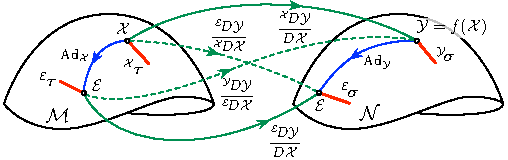
\includegraphics{figures/jacobians_adjoints}
\caption{函数 $\cY=f(\cX)$ 中所有切空间之间的线性映射,从 $\cM$ 到 $\cN$。线性映射 ${{^\cE}\!\bftau=\Ad[\cM]{\cX}\,{^\cX}\!\bftau}$, ${{^\cE}\!\bfsigma=\Ad[\cN]{\cY}\,{^\cY}\!\bfsigma}$, ${{^\cE}\!\bfsigma=\ldpar{\cY}{\cX}\,{^\cE}\!\bftau}$,并且 ${{^\cY}\!\bfsigma=\rdpar{\cY}{\cX}\,{^\cX}\!\bftau}$,形成一个指向方程 \eqRef{equ:derivatives_lr_adjoints} 的循环(实线)。交叉的Jacobian矩阵(虚线)形成了更多的映射循环,导致方程 (\ref{equ:derivatives_ex_adjoints},\ref{equ:derivatives_ye_adjoints})。} 
\label{fig:jacobians_adjoints}
\end{figure}

我们可以从方程 (\ref{equ:Adj1}, \ref{equ:lin_approx}, \ref{equ:lin_approx_left}) (参见 \figRef{fig:jacobians_adjoints}) 中展示左和右Jacobian矩阵由 $\cM$ 和 $\cN$ 的伴随相关联的关系,
%
\begin{align}\label{equ:derivatives_lr_adjoints}
\ldpar{f(\cX)}{\cX}\Ad[\cM]{\cX} = \Ad[\cN]{f(\cX)}\rdpar{f(\cX)}{\cX} 
~.
\end{align}


%=======================================================
\subsubsection{交叉使用右--左Jacobian矩阵}

也可以同时使用右侧加号和左侧减号来定义Jacobian矩阵,反之亦然。
虽然不太可能,但它们有时很有用,因为它们将局部的正切映射到全局的正切,反之亦然。
简而言之,我们将通过伴随把它们与其它Jacobian矩阵联系起来,
%
\begin{align}
\lrdpar{\cY}{\cX} &= \lldpar{\cY}{\cX}\,\Ad{\cX} ~~~\,= \Ad{\cY}\,\rrdpar{\cY}{\cX} \label{equ:derivatives_ex_adjoints}\\
\rldpar{\cY}{\cX} &= \rrdpar{\cY}{\cX}\,\Ad{\cX}\inv = \Ad{\cY}\inv\,\lldpar{\cY}{\cX}\label{equ:derivatives_ye_adjoints}
~,
\end{align}
%
其中 $\cY=f(\cX)$ 。现在,上一行和下一行的上标表明表示微分的参考坐标系。
相应的小 $\bftau$ 的近似值取为,
%
\begin{align}
f(\cX\op{^\cX}\bftau) 
 &\xrightarrow[{^\cX\!\bftau}\to0]{} \lrdpar{f(\cX)}{\cX}\,{^\cX}\bftau \op f(\cX) \label{equ:lin_approx_rl}\\
f({^\cE}\bftau\op\cX) 
 &\xrightarrow[{^\cE\!\bftau}\to0]{} f(\cX) \op \rldpar{f(\cX)}{\cX}\,{^\cE}\bftau \label{equ:lin_approx_lr}
 ~.
\end{align}



%%%%%%%%%%%%%%%%%%%%%%%%%%%%%%%%%%%%%%%%%
\subsection[Uncertainty, covariances]{流形中的不确定性与协方差传播}

我们定义局部扰动 $\bftau$ 为在切向量空间 $\mtanat{\cM}{\bar\cX}$ 中围绕着点 $\bar\cX\in\cM$ 的扰动,使用右结合(right-)的 $\op$ 和 $\om$,
%
\begin{align}\label{equ:uncertainty}
\cX &= \bar\cX \op \bftau~, & \bftau &=\cX \om \bar\cX ~\in\mtanat{\cM}{\bar\cX}
~.
\end{align}
%
协方差矩阵可以通过标准期望算子 $\bbE[\cdot]$ 在 $\bar\cX$ 处的切空间上正确定义,
%
\begin{align}\label{equ:cov}
\bfSigma_\cX \te \bbE[\bftau\bftau\tr] = \bbE[(\cX \om \bar\cX)(\cX \om \bar\cX)\tr]~\in\bbR^{m\times m}
~,
\end{align}
%
这允许我们定义流形上的高斯变量, $\cX\sim\cN(\bar\cX,\bfSigma_\cX)$,参见 \figRef{fig:covariance}。
注意,虽然我们写 $\bfSigma_\cX$,但协方差还是正切扰动 $\bftau$ 的协方差。
由于 $\mtan{\cM}$ 的维度 $m$ 与 $\cM$ 的自由度相匹配,因此这些协方差被很好地定义。%
%
\footnote{%
一个幼稚的定义 $\bfSigma_\cX \te \bbE[(\cX - \bar\cX)(\cX - \bar\cX)\tr]$ 总是错误的定义,如果 $\mathrm{size}(\cX)>\dim(\cM)$,这是大多数非平凡流形的情况。%
}

\begin{figure}[tb]
\centering
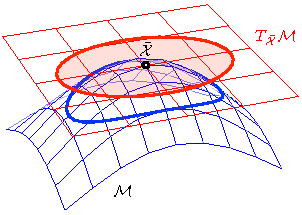
\includegraphics{figures/covariance}
\caption{围绕着点 $\bar\cX\in\cM$ 的不确定性被正确地表示为该点(红色)处向量空间的正切协方差。
使用 $\op$ 方程 \eqRef{equ:uncertainty},在切空间中的概率椭圆被缠绕在流形上(蓝色),从而说明了群上的概率集中区域。}
\label{fig:covariance}
\end{figure}




扰动也可以在全局参考中表示,即在原点 $\mtanat{\cM}{\cE}$ 处的切空间中,
使用左结合(left-)的 $\op$ 和 $\om$,
%
\begin{align}\label{equ:uncertainty_left}
\cX &= \bftau\op\bar\cX~, & \bftau &=\cX \om \bar\cX ~\in\mtanat{\cM}{\cE}
~.
\end{align}
%
这允许使用在方程 \eqRef{equ:cov} 中的左结合(left-)减号的协方差矩阵的全局规范。
例如,一个三维方向已知是在水平面中的旋转,可以与协方差矩阵 $^\cE\bfSigma=\diag(\sigma_\phi^2,\sigma_\theta^2, \infty)$ 相关联。
因为“水平(horizontal)”是一个全局规范,因此必须在全局参考中指定 $^\cE\bfSigma$ 。

%最后请注意,在这最后一点上没有达成共识。
%当文献 \cite{forster2017-TRO} 和我们使用局部扰动 $\cX=\bar\cX\op{^\cX\!\bftau}$ 时,文献 \cite{EADE-Lie,BARFOOT-14} 使用围绕原点的扰动, $\cX={^\cE\!\bftau}\op\bar\cX$,产生全局协方差规范。
因为全局扰动和局部扰动是由伴随方程 \eqRef{equ:Adj2} 联系起来的,它们的协方差的变换可以用
%
\begin{align}
^\cE\bfSigma_{\cX} = \Ad[\cM]{\cX} \, ^\cX\bfSigma_{\cX} \, \Ad[\cM]{\cX}\tr
~.
\end{align}

协方差的传播通过函数 $f:\cM\to\cN;\cX\mapsto \cY=f(\cX)$ 只需要用Jacobian矩阵方程 \eqRef{equ:Jacobian} 线性化方程 \eqRef{equ:lin_approx} 以获得熟悉的公式,
%
\begin{align}\label{equ:cov_propagation}
\bfSigma_{\cY} \approx \ndpar{f}{\cX} \, \bfSigma_\cX \, \ndpar{f}{\cX}\tr
~\in\bbR^{n\times n}
~.
\end{align}



%%%%%%%%%%%%%%%%%%%%%%%%%%%%%%%%%%%%%%%
\subsection{流形上的离散积分}

指数映射 $\cX(t)=\cX_0\circ\Exp(\bfv t)$ 执行恒定速度 $\bfv\in\mtanat{\cM}{\cX_0}$ 的连续时间积分到流形上。
非恒定速度 $\bfv(t)$ 通常通过将它们分割成分段恒定小量 $\bfv_k\in\mtanat{\cM}{\cX_{k-1}}$,(短的)持续时间为 $\dt_k$,并写成离散积分来处理
%
\begin{align*}
\cX_k &= \cX_0\circ\Exp(\bfv_1 \dt_1)\circ\Exp(\bfv_1 \dt_2)\circ\cdots\circ\Exp(\bfv_k \dt_k) \\
 &= \cX_0 \op \bfv_1 \dt_1\op\bfv_1 \dt_2\op\cdots\op\bfv_k \dt_k
~.
\end{align*}
%
等价地(\figRef{fig:manifold_int}),我们可以定义 $\bftau_k=\bfv_k\dt_k$ 并
将积分构造为(小的)离散正切步 $\bftau_k\in\mtanat{\cM}{\cX_{k-1}}$ 的 ``总和(sum)'',即,
%
$
\cX_k \te \cX_0\op\bftau_1\op\bftau_2\op\cdots\op\bftau_k.
$
%
我们用递归的形式写出所有这些变体,
%
\begin{align}\label{equ:int_recursive}
\cX_k = \cX_{k-1}\op\bftau_k = \cX_{k-1}\circ\Exp(\bftau_k) = \cX_{k-1}\circ\Exp(\bfv_k\dt_k)
~.
\end{align}
%

\begin{figure}[tb]
\centering
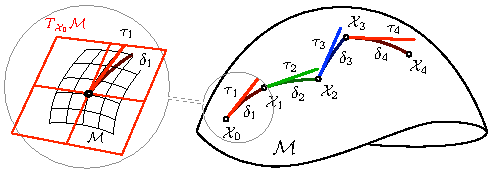
\includegraphics{figures/manifold_int}
\caption{流形上的运动积分。每一个运动数据生成一个步长 $\bftau_k\in\mtanat{\cM}{\cX_{k-1}}$,该步长被缠绕为局部运动增量或 `delta' $\delta_k=\Exp(\bftau_k)\in\cM$,然后与 $\cX_{k-1}$ 组合以产生 $\cX_k=\cX_{k-1}\circ\delta_k=\cX_{k-1}\circ\Exp(\bftau_k)=\cX_{k-1}\op\bftau_k\in\cM$.}
\label{fig:manifold_int}
\end{figure}%

常见的例子是将三维角速度 $\bfomega$ 积分到旋转矩阵, $\bfR_k=\bfR_{k-1}\Exp(\bfomega_k\dt)$,或积分到四元数 $\bfq_k=\bfq_{k-1}\Exp(\bfomega_k\dt)$。

